\section{WC 25/11/24}

\subsection*{Overview:}
With a note mapping system researched, designed, and a prototype built, I decided to dedicate this week to exploring various notetaking methods, including both typing and handwritten, to expand on my initial research into effective notetaking strategies.

\subsection*{Achievements, Thoughts and Ideas:}
I approached this week having a strong idea for what I wanted to (and I knew was possible to) build as a tool to present my research. I knew it was now crucial that I fully understood what I wanted to achieve and the huamn thought patterns I wanted to address to achieve this. 

So far my understanding of notetaking methods was sourced primarily from my research of techniques and expanded by my own personal findings and theorised best practises, however I hadn't yet explored the vast depth of research completed by more scientific approaches. I decided to use JSTOR within the school library to help me find some fascinating articles which I could learn from:

Firstly I read back over my past notes and revisited  my requirement for handwritten notes to be supported by the software. I had always felt that longhand forms of data recording aided my ability to recall information (and is crucial for those in the education system) but I wanted to verify this gut feeling. I came across \nameref{research:WritingVsTyping} (later built on by \nameref{research:WritingVsTyping2}) which used a large data set of students to confirm my beliefs. This week I chose to handwrite my research notes to fit with my findings and ensure I was able to apply my learnings to my own work.

I wanted to try and find scientific confirmation that my 'mind map' centred philosophy regarding the storage of information was in fact an ideal solution, whilst also being careful to avoid confirmation bias. This article is a much less formal document however gives a more "grounded" insight from a group of teachers who discuss the impacts of such notetaking techniques on their students. I found \nameref{research:StructuredNoteTaking} to be a fascinating read, it confirmed my beliefs that a more structured approach to notetaking is beneficial, however it also highlighted the importance of flexibility within this structure to allow for personalisation. This was something I had not yet considered and will be crucial to implement within my software.
Having completed this weeks research pieces (\nameref{research:WritingVsTyping}, \nameref{research:WritingVsTyping2}, \nameref{research:StructuredNoteTaking}, \nameref{research:NotetakingReview},\nameref{research:StrategicNotetaking}, \nameref{research:LaptopVsLonghandSummary}) I have come away with some conclusions. It has been unanimously agreed by all that laptop (typed) notetakers copy lecture / course content far more directly and record more information, while this is beneficial for creating thorough notes this does skip the 'encoding' step of notetaking. This step causes the brain to rephrase / reframe ideas to simplify recording by longhand (a much slower recording technique at average 28WPM vs typists around 60). While less detail is recorded and notes are harder to later reference it seems that this encoding effect can contribute to huge academic performance gains as the content is more clearly stored in the students mind making longhand notetaking a far more beneficial strategy for students. 

Whilst clearly longhand notetaking is the superior method, it is not without its flaws. The most obvious being the speed of recording, this can lead to students missing key points or being unable to keep up with the pace of a lecture. This is where I believe my software can come into play, by allowing students to quickly jot down key points and then later expand on them in their own time, they can benefit from the encoding effect while also ensuring they don't miss out on important information.


\subsection*{Power of Three:}
\textbf{This week's Tasks laid out per day}

\begin{tabularx}{\textwidth}{
  >{\raggedright\arraybackslash}X  % First column expands
  >{\centering\arraybackslash}p{1.5cm}  % Middle column has fixed width
  >{\raggedright\arraybackslash}X  % Third column expands
}
\toprule
\textbf{Goal} & \textbf{Achieved?} & \textbf{Notes} \\
\midrule

\rowcolor{gray!10}
\multicolumn{3}{l}{\textbf{Monday}} 

\\ Explore prior thoughts around typed notes vs handwritten mediums & \ding{51} &  \\
Complete last week's diary entries with most recent prototypes & \ding{51} & \\
Update UX design research with example images I found browsing internet & \ding{51} & \\

\rowcolor{gray!10}
\multicolumn{3}{l}{\textbf{Tuesday}} \\
Research note layout methods  & \ding{51} & \\
Search for resources around digitally written notes vs paper written notes & \ding{55} & Resources found but not yet explored\\



\rowcolor{gray!10}
\multicolumn{3}{l}{\textbf{Thursday}} \\
Analyse e-inked notes & \ding{51} & \\
 Continue to write-up of other research notes & \ding{51} & \\
Plan the following week's tasks & \ding{51} &  \\




\rowcolor{gray!10}
\multicolumn{3}{l}{\textbf{Friday}} \\
Find new resources I can use during the EPQ library session& \ding{51} &Whilst much of the technical research was best sourced online, and the scientific reports were difficult to get hold of in paper form, found a section in the library containing books about teaching, exam and student learning methods to be highly useful to inform my project (please see \autoref{diary:library-section}) \\
Explore online resources I could access & \ding{51} & Whilst I had already been using JSTOR for my research I found out about school subscriptions to Oxford academic resources and Springer Journals articles\\
Speak to mentor about expanding previous research pieces when I wish to dive deeper into a topic at a later date
 & \ding{51} & My mentor recommended doing this and to list when certain aspects are added clearly in my diary and in the research piece so that a clear timeline of events can be formed
\\




\bottomrule
\end{tabularx}

\begin{figure}
\centering
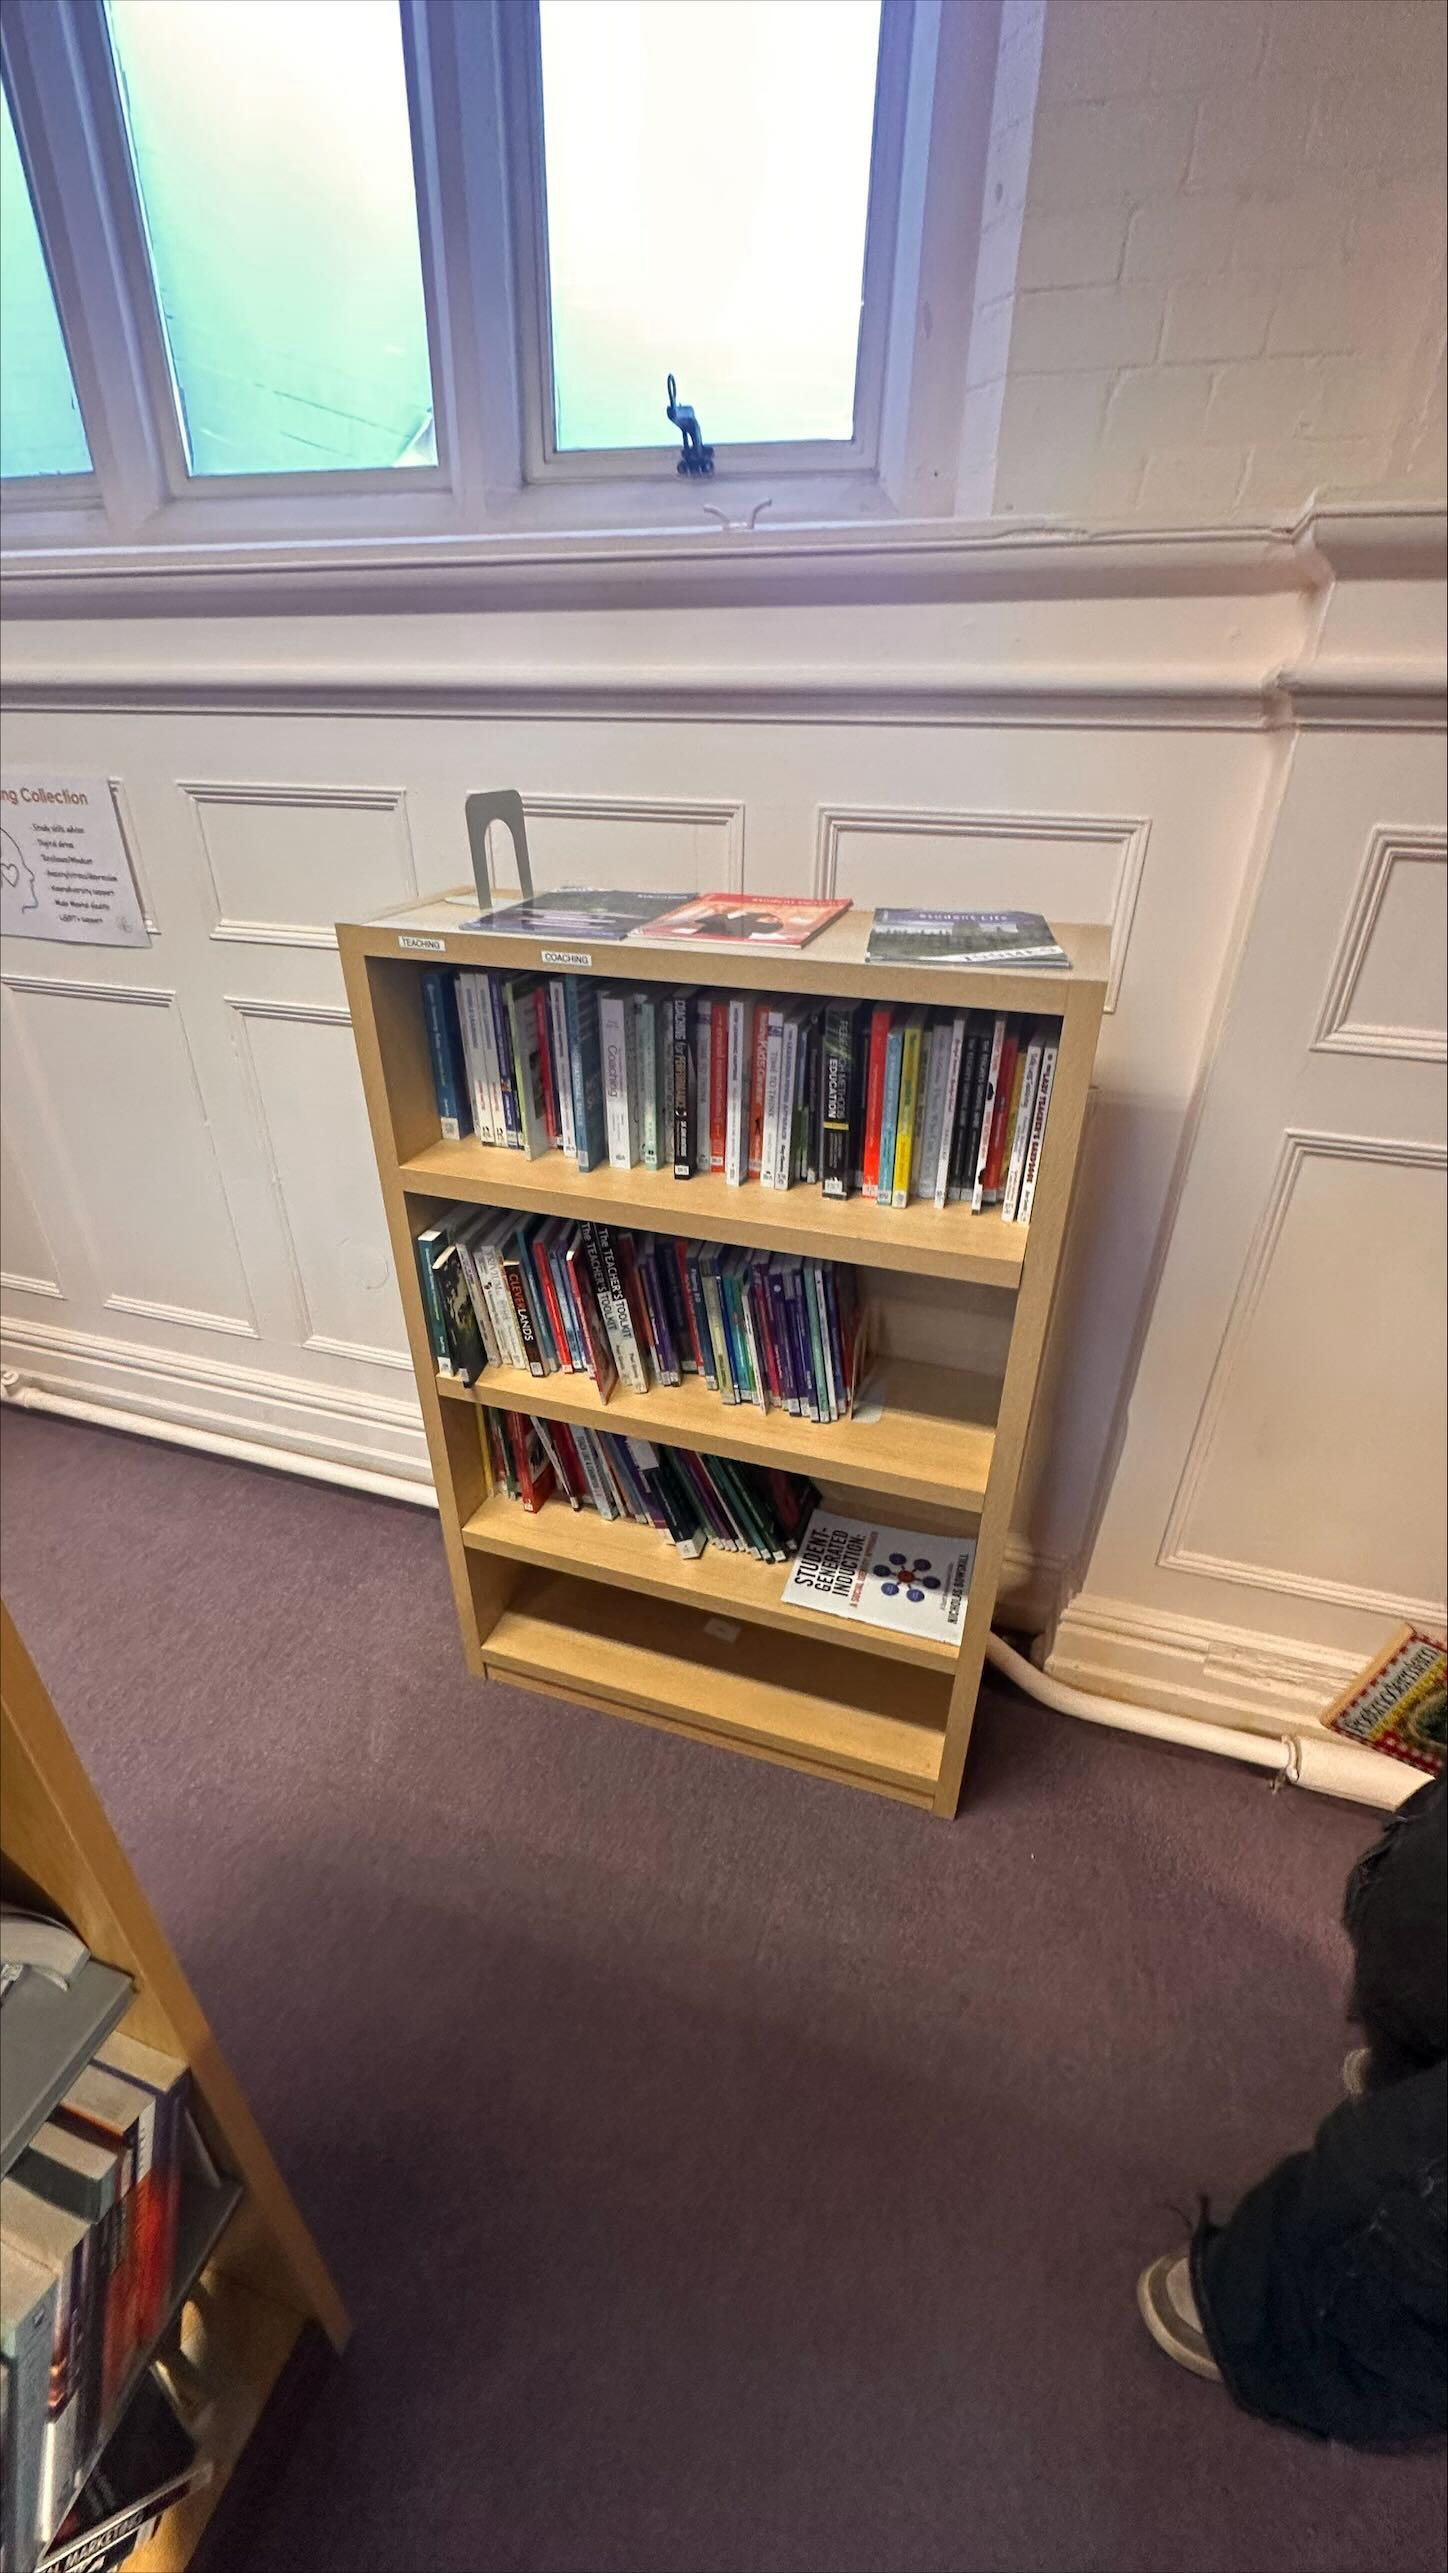
\includegraphics[width=0.4\textwidth]{Diary/9_WC_25-11-24/media/library.png}
\caption{A useful section of the library I have identified for future research}
\label{diary:library-section}
\end{figure}

\subsection*{What did I learn?}
This week I gained a lot of knowledge regarding not just what the best methods for learning are but also why they are so effective, my new understanding of this knowledge will enable me to maximise my final software's abilities

\subsection*{Plans for next week:}
Next week I want to explore how I will implement these learnings, I know have what I want to achieve, and how I can technically make that happen; I need to understand how I marry those two ideas together
